\documentclass{article}
\usepackage{hyperref}
\usepackage{graphicx}

\title{RevNets}
\author{Filip\\ \texttt{f@filip.world}}

\begin{document}
\maketitle

\begin{abstract}
  Smart contracts have enabled new models for organization and governance, but have in some ways failed to deliver on the promise of truly decentralized coordination. Among other causes, this is often due to the challenge of bootstrapping an organization while creating a product. The centralized nature of this process often leaves the founding team or core developers with little incentive to distribute power by the time a community has been formed. This leaves both parties worse-off: founders must contend with the day-to-day overhead of running a DAO or a governance system which has little to do with their end product, and participants must contend with the risk of misalignment, rugpulls, and scams. \textbf{RevNets} are a new model for creating, scaling, and operating decentralized networks according to pre-defined economic incentives which align participants and remove the need for governance, freeing founders from day-to-day management and making rugpulls impossible.
\end{abstract}

\section{Introduction}

Ethereum.org\cite{daos} describes DAOs as ``Member-owned communities without centralized leadership.''

\begin{quote}
  \textit{DAOs allow us to work with like-minded folks around the globe without trusting a benevolent leader to manage the funds or operations.}
\end{quote}

DAOs and other onchain organizations often fail to live up to the promise of collective ownership and governance. Despite the use of theoretically decentralized consensus models, funding decisions are often made by a founding team or group of core developers. In practice, governance frequently serves only to ratify decisions which have already been made. This can lead to voter apathy and community disengagement.

Smart contracts have enabled novel models for organizing, operating, and governing communities through incentives, but current implementations are often bottlenecked by a core team required to facilitate

\section{Mechanism}

Each RevNet has its own token (the \textit{network token}) which represents partial network ownership. Anyone can pay ETH into a network to buy its token (thus joining the network). Under the network's initial conditions, payers receive 1 token per ETH.\footnote{For simplicity's sake, this section assumes a RevNet is using ETH-based accounting. For a clearer understanding of USD-based accounting, see Section~\ref{sec:accounting_types}.}

A RevNet's token issuance evolves over generations which last a pre-defined length of time (28 days, for example). Three parameters determine how its tokens are issued:

\begin{itemize}
  \item \textbf{The Entry Curve}. The cost to enter the network increases over time, incentivizing people to join sooner. The entry curve defines how much more expensive tokens become each generation. With a 5\% entry curve, 5\% fewer tokens are minted per ETH each generation.
  \item \textbf{The Exit Curve}. Leaving the network (by burning tokens) reclaims some ETH from the network. The closer an exit curve is to 100\%, the more ETH goes to the last participants to exit, and less ETH goes to the first participants to exit. This incentivizes participants to stay in the network longer. You can visualize and experiment with different exit curves on Desmos.
  \item \textbf{The Boost}. For a pre-determined length of time (140 days, for example) after a RevNet's creation, a percentage of newly generated tokens are allocated to a specific address. This address could be a developer multisig, a staking rewards contract, an airdrop stockpile, or something else. When the boost period ends, this allocation drops to 0.
\end{itemize}

Network creators can optionally pre-mint a number of tokens for themselves at the time of the network's creation. RevNets have no owner. Once they are deployed, their parameters are locked in place. Funds can only leave the network when people exit.

\subsection{Entry Curve}

The entry curve can be expressed as:

\begin{equation}
  T_n = T_0 \times (1 - r)^{(n - 1)}
\end{equation}

where:
\begin{itemize}
  \item $T_n$ is the number of tokens issued per ETH in the $n^{th}$ generation,
  \item $T_0$ is the number of tokens issued per ETH in the initial generation,
  \item $r$ is the \textit{Entry Curve}, or rate of decrease per generation (expressed as a decimal), and
  \item $n$ is the generation number, which increments sequentially starting from 1.
\end{itemize}

Since RevNets always have a $T_0$ (initial price) of 1 token per ETH, this can be re-written as:

\begin{equation}
  T_n = (1 - r)^{(n - 1)}
\end{equation}

\begin{figure}[h]
  \centering
  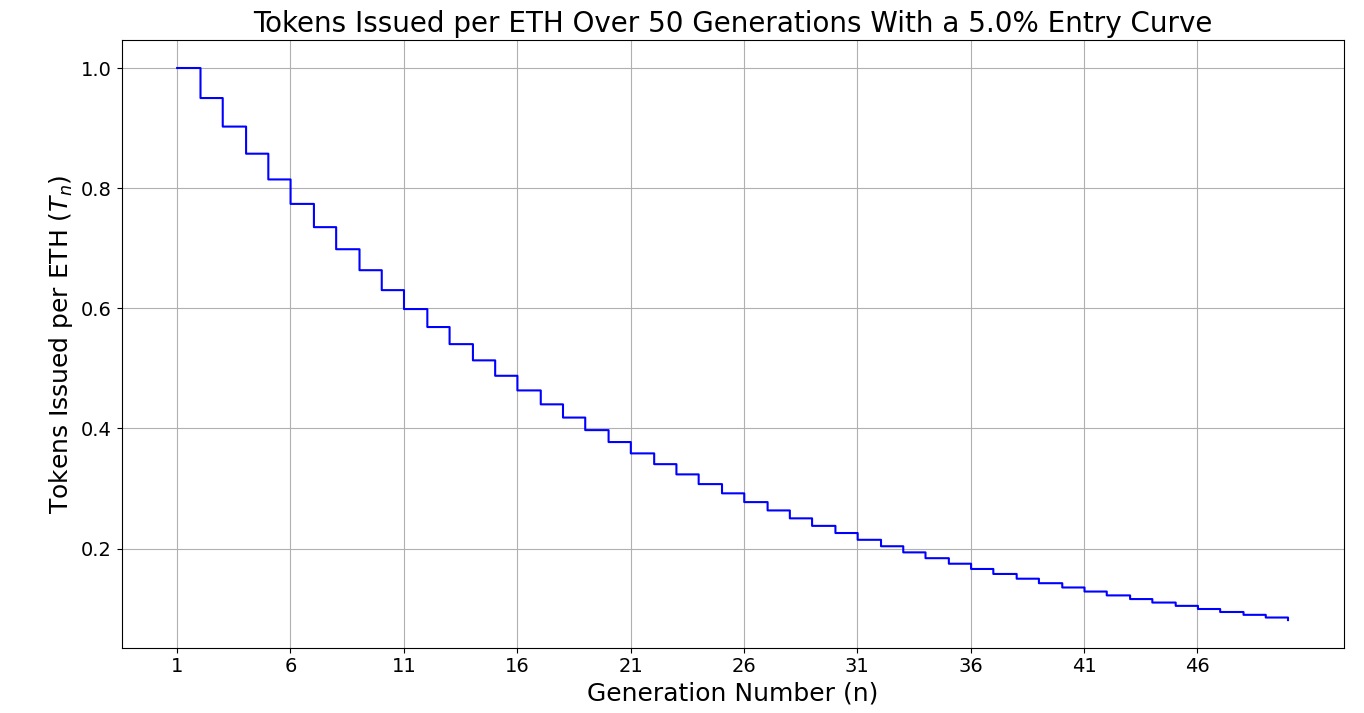
\includegraphics[width=\textwidth]{figures/single-entry-curve.png}
   \caption{This figure shows how $T_n$ (the number of tokens issued per ETH in the $n^{th}$ generation) varies across 50 generations with a 5\% entry curve $(r = 0.05)$. Note that $T_n$ decreases rapidly at first, then more gradually as $T_n$ tends towards 0 over many generations. Put simply, the tokens get more expensive over time.}
\end{figure}

\begin{figure}[h]
  \centering
  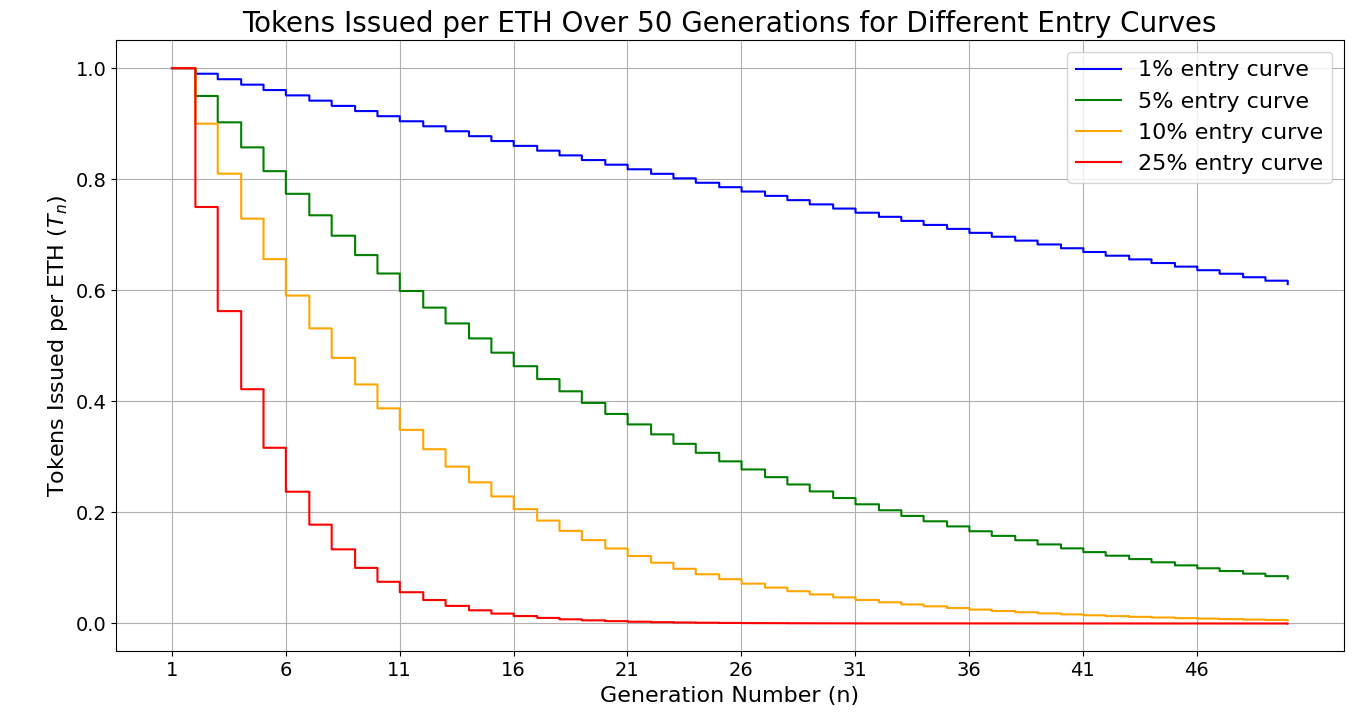
\includegraphics[width=\textwidth]{figures/multi-entry-curves.png}
  \caption{This figure shows how $T_n$ varies over 50 generations with 1\%, 5\%, 10\%, and 25\% entry curves $(r = 0.01, 0.05, 0.1, 0.25)$. Note that for greater entry curves, $T_n$ tends towards 0 more quickly.}
\end{figure}

\subsection{Exit Curve}

\subsection{Boost}

\section{Implementation}

Our implementation extends the Juicebox protocol

To create a RevNet, one must define

\section{Applications}

\subsection{Software}

\subsection{Social Networks}

\section{Miscellanea}

\subsection{Network Token Implementation}

\subsection{Accounting Types}\label{sec:accounting_types}

If the network uses USD-based accounting, payers will receive 1 token per USD worth of ETH under the network's intial conditions. For instance, if the ETH price is 1,000 USD, paying 1 ETH into the network will yield 1,000 tokens.

\section{Conclusion}

\bibliographystyle{plain}
\bibliography{references}

\end{document}

